\documentclass{article}

\usepackage[a4paper, total={6in, 8in}]{geometry}
\usepackage[utf8]{inputenc}
\usepackage{amsmath}
\usepackage{amssymb}
\usepackage{tabularx}
\usepackage[makeroom]{cancel}
\usepackage{arydshln}
\usepackage{graphicx}
\usepackage{fancyhdr}
\usepackage{enumitem}
\usepackage{multirow}
\usepackage{amsfonts}

\newcommand{\overbar}[1]{\mkern 1.5mu\overline{\mkern-1.5mu#1\mkern-1.5mu}\mkern 1.5mu}

\pagestyle{fancy}
\fancyhf{}
\lhead{John J Li}
\rhead{CSE120 Spring 2021 Homework 6}
\rfoot{\thepage}
\lfoot{April 2021} 
\renewcommand{\headrulewidth}{0.4pt}
\renewcommand{\footrulewidth}{0.4pt}

\setlength{\parskip}{1em}
\setlength\parindent{0px}
\title{CSE120 Spring 2021 Homework 6}
\date{\today}
\author{John J Li}

\begin{document}
    \maketitle
    \thispagestyle{empty}
    \noindent\rule{\textwidth}{0.8pt}

    %###################################################################################

    \section*{Problem 1}

    Answer the following questions for a synchronous machine with the following state 
    transition table with one input X and one output Z.

    \begin{center}
        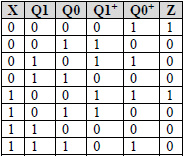
\includegraphics[scale=0.75]{CSE120_HW6_01_Question.jpg}
    \end{center}

    (a) Is this is Moore or Mealy machine?

    \begin{enumerate}[label=\textbf{Solution:}, leftmargin=*]
        \item 
        This is a Moore machine.
    \end{enumerate}

    (b) Create the state transition diagram.

    \textbf{Solution:}

    \begin{center}
        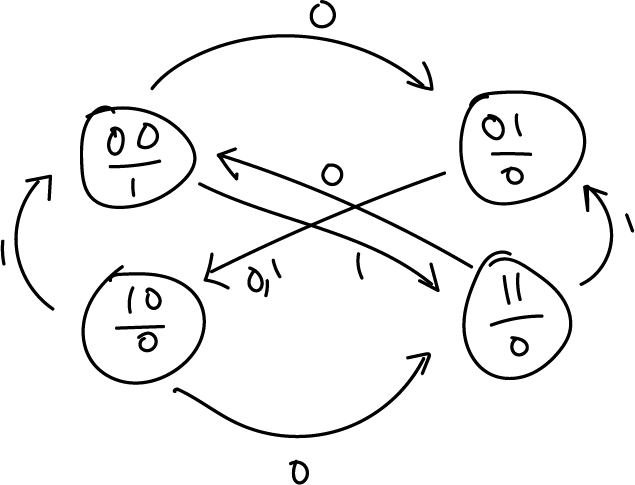
\includegraphics[scale=0.3]{Q1_b1.png}
    \end{center}

    (c) Design a system using T flip flops and NAND gates only. Include all K-maps and a 
    final circuit diagram.
    
    \textbf{Solution:}

    \begin{center}
        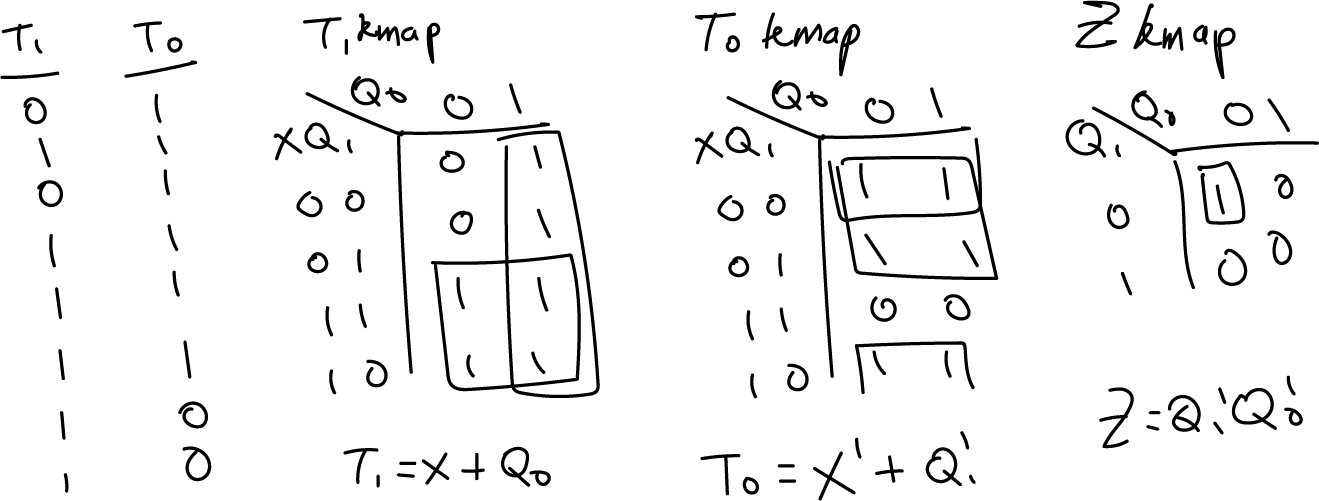
\includegraphics[width=\linewidth]{Q1_Kmaps.png}
    \end{center}

    \begin{center}
        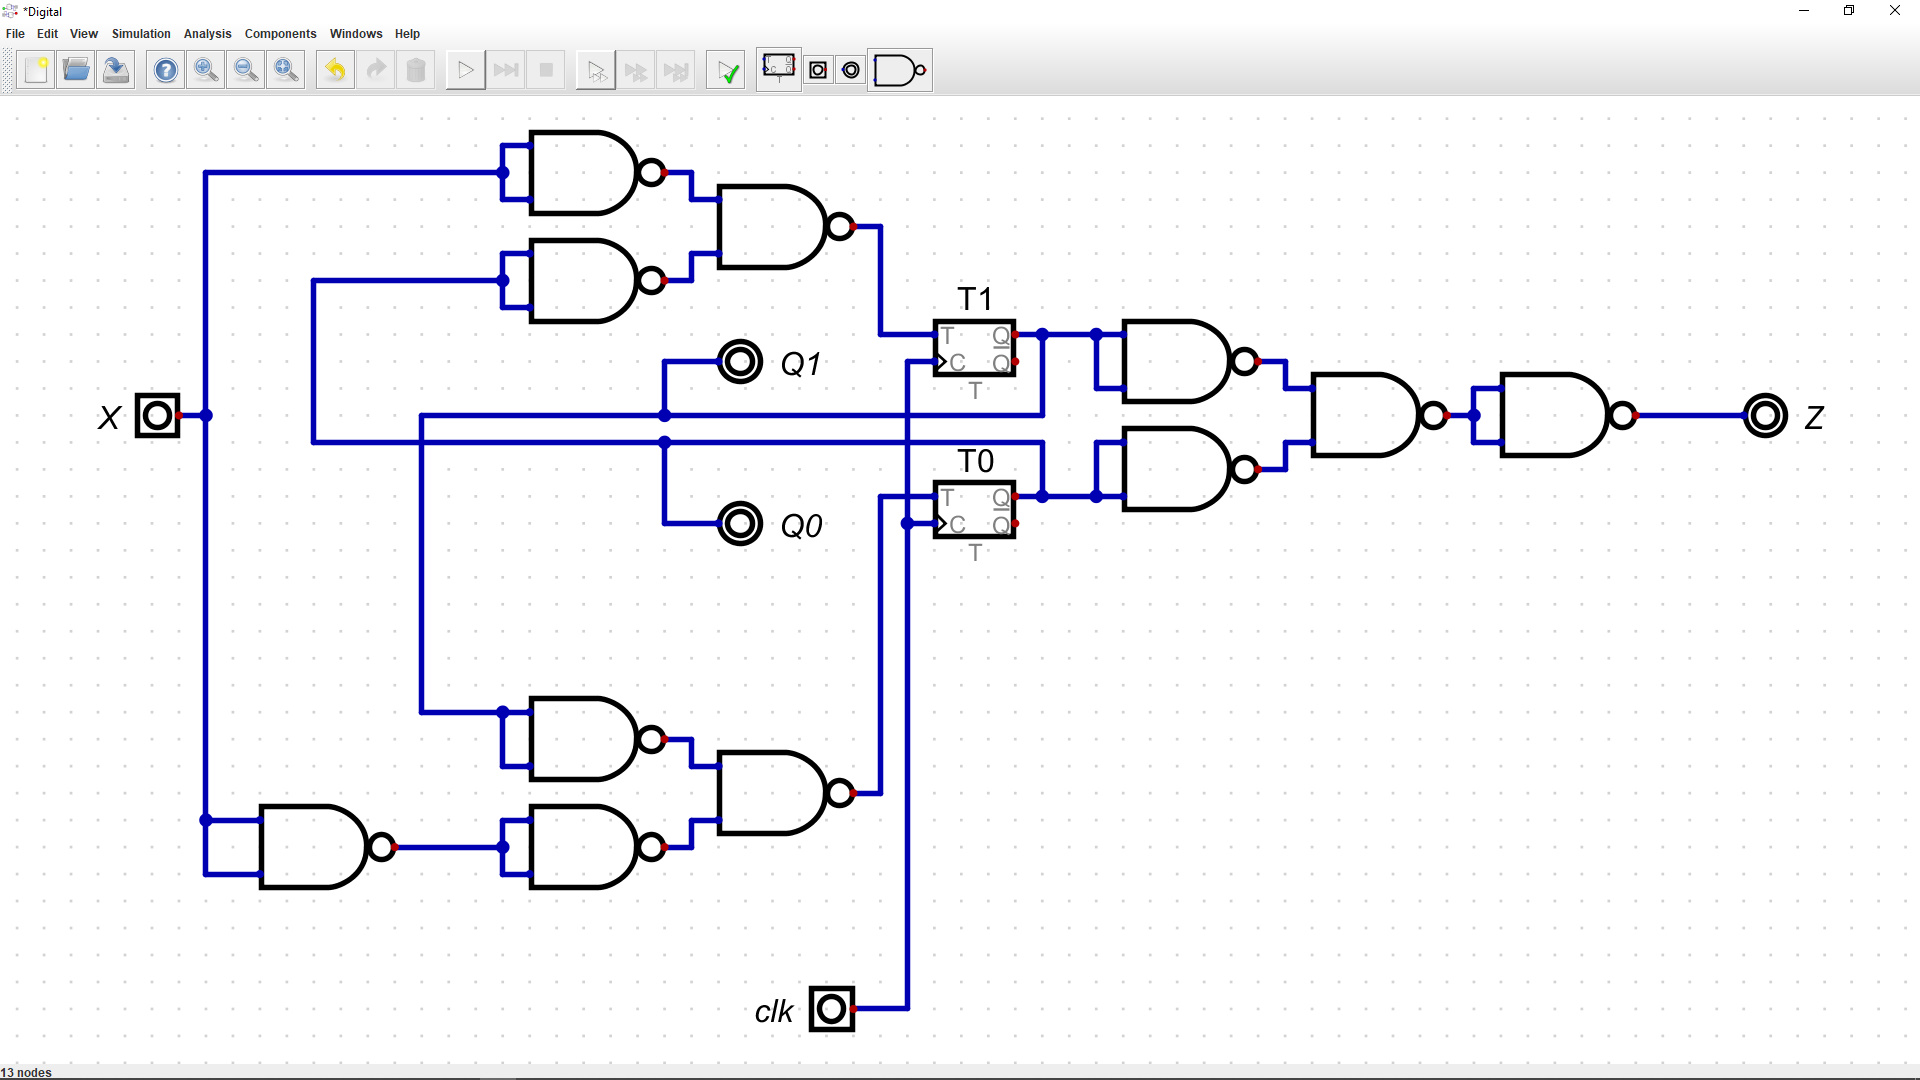
\includegraphics[width=\linewidth]{Q1_c2.jpg}
    \end{center}

    %###################################################################################

    \section*{Problem 2}

    Show a state diagram for a Mealy system, the output of which is 1 if and only if the 
    pattern 1 1 0 1 has occurred immediately after a 0. Assume overlapping is allowed 
    (the final 1 in the pattern can be considered the first one in the next sequence). 
    A sample input/output trace and the minimum number of states required is shown.

    \begin{center}
        x 0 0 1 1 0 1 1 0 1 1 0 1 1 1 0 1 1 0 1 1 0 1

        z 0 0 0 0 0 1 0 0 1 0 0 1 0 0 0 0 0 0 1 0 0 1 0 0
    \end{center}

    \textbf{Solution:}

    \begin{center}
        \begin{tabular} {c|l}
            State & State Description \\
            \hline
            $S_1$ & Initial 0; reset 0 \\
            $S_2$ & 1 after a 0 \\
            $S_3$ & 2 repeating 1s \\
            $S_4$ & 110 in sequence \\
            $S_5$ & 3 or more repeating 1s
        \end{tabular}
    \end{center}

    \begin{center}
        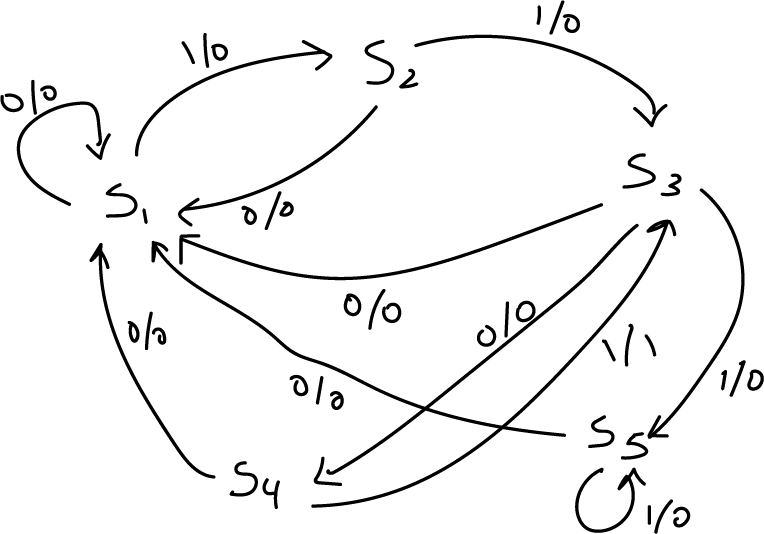
\includegraphics[scale=0.3]{Q2_state_diagram.png}
    \end{center}

    %###################################################################################

    \section*{Problem 3}

    Design a system with one input called “Up” such that when “Up” equals 1, the machine 
    counts 1, 2, 3, 4, 5 and repeat. If the “Up” input equals 0, the machine counts down 
    5, 4, 3, 2, 1 and repeat.

    Show the State Transition Diagram, State Transition table, K-maps, and Minimum SOP 
    equations assuming D flip flops and AND/OR/NOT combinational logic. Make sure to 
    indicate on your State Transition Diagram what happens if the system initially is in 
    one of the unused states 0, 6, or 7 (Do NOT make any assumptions, use your D 
    equations to figure out the state transitions).

    \textbf{Solution:}

    \begin{center}
        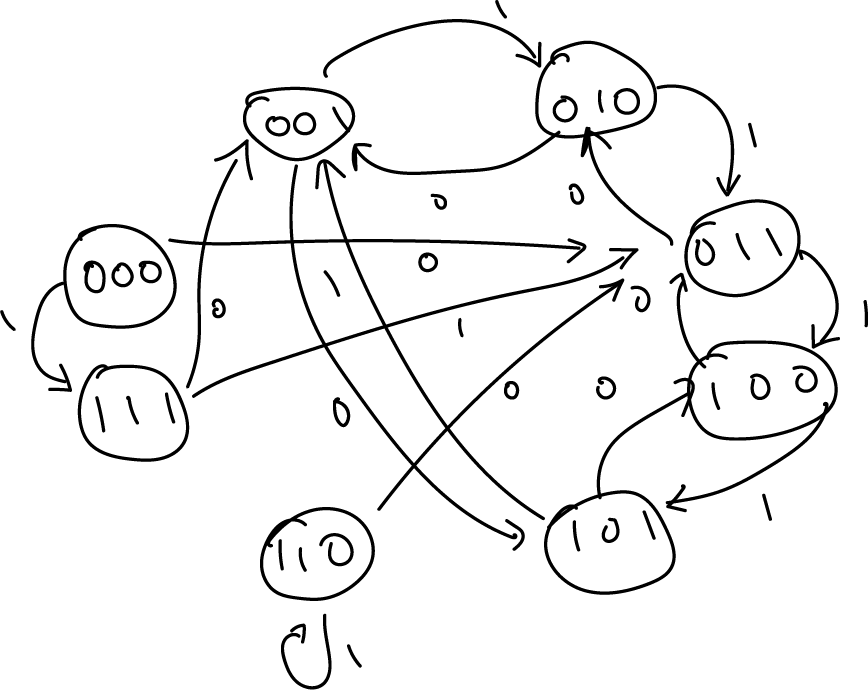
\includegraphics[scale=0.3]{Q3_State_Diagram.png}
    \end{center}

    \begin{center}
        \begin{tabular} {c|ccc|ccc}
            Up & $Q_2$ & $Q_1$ & $Q_0$ & $Q_2^+$ & $Q_1^+$ & $Q_0^+$ \\
            \hline
            0 & 0 & 0 & 0 & X & X & X \\
            0 & 0 & 0 & 1 & 1 & 0 & 1 \\
            0 & 0 & 1 & 0 & 0 & 0 & 1 \\
            0 & 0 & 1 & 1 & 0 & 1 & 0 \\
            0 & 1 & 0 & 0 & 0 & 1 & 1 \\
            0 & 1 & 0 & 1 & 1 & 0 & 0 \\
            0 & 1 & 1 & 0 & X & X & X \\
            0 & 1 & 1 & 1 & X & X & X \\
            \hdashline
            1 & 0 & 0 & 0 & X & X & X \\
            1 & 0 & 0 & 1 & 0 & 1 & 0 \\
            1 & 0 & 1 & 0 & 0 & 1 & 1 \\
            1 & 0 & 1 & 1 & 1 & 0 & 0 \\
            1 & 1 & 0 & 0 & 1 & 0 & 1 \\
            1 & 1 & 0 & 1 & 0 & 0 & 1 \\
            1 & 1 & 1 & 0 & X & X & X \\
            1 & 1 & 1 & 1 & X & X & X \\
        \end{tabular}
    \end{center}

    \begin{center}
        \begin{tabular} {c|c}
            Q & Flip Flop \\
            \hline
            $Q_0$ & $D_0$ \\
            $Q_1$ & $D_1$ \\
            $Q_2$ & $D_2$ \\
        \end{tabular}
    \end{center}

    \begin{center}
        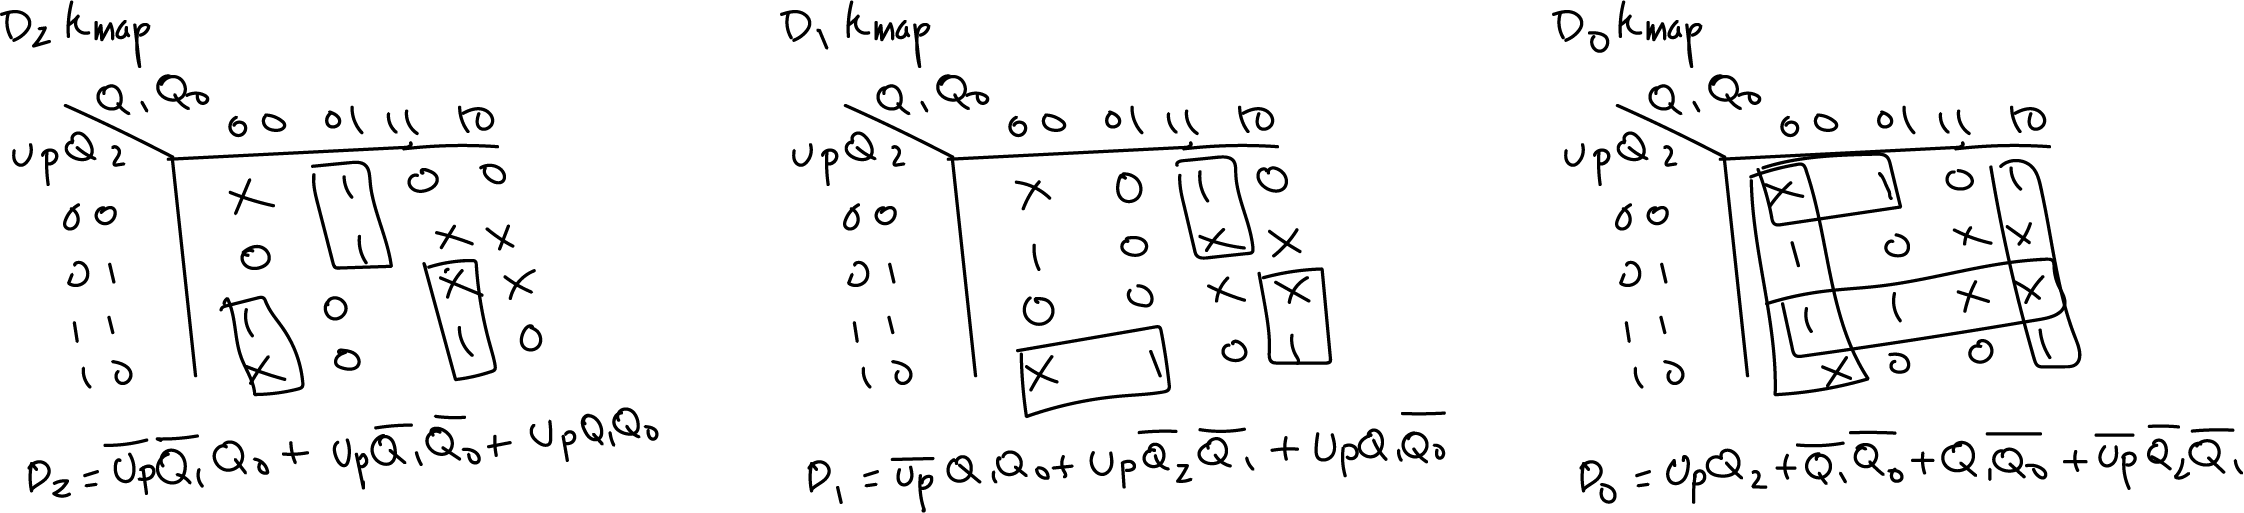
\includegraphics[width=\linewidth]{Q3_Kmaps.png}
    \end{center}

    %###################################################################################

    \section*{Problem 4}

    Using the following state transition diagram with 6 states $(Q_2Q_1Q_0)$ with 1 
    input, X, and 1 output, Z:

    \begin{center}
        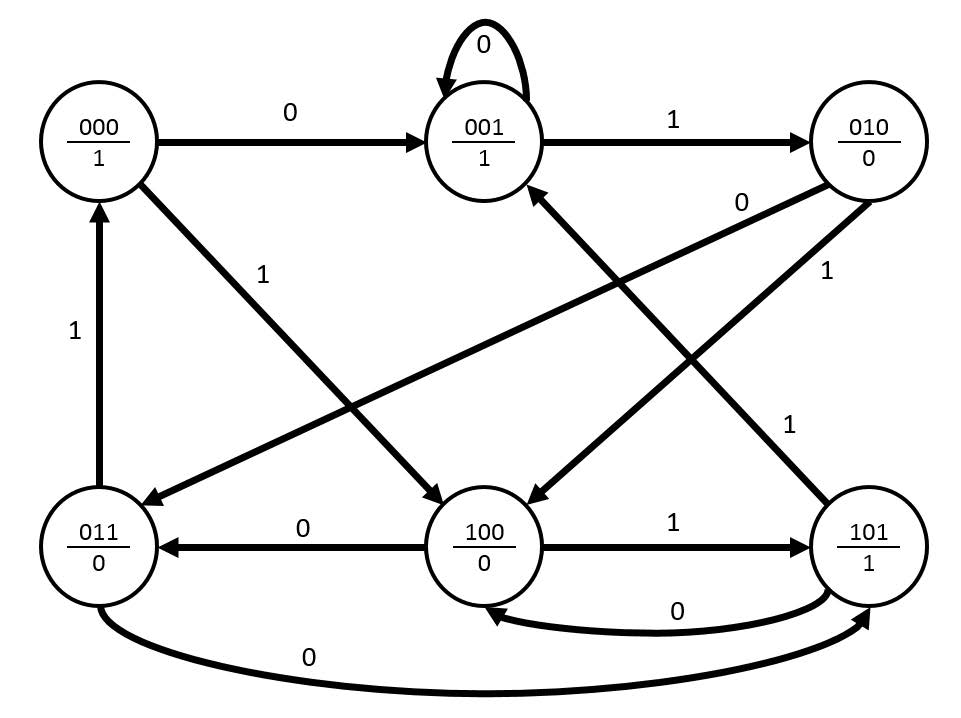
\includegraphics[scale=1]{Q4_Question.jpg}
    \end{center}

    a) Create the state transition table.

    \textbf{Solution:}

    \begin{center}
        \begin{tabular} {c|c|ccc|ccc|c}
            \# & X & $Q_2$ & $Q_1$ & $Q_0$ & $Q_2^+$ & $Q_1^+$ & $Q_0^+$ & Z \\
            \hline
            0 & 0 & 0 & 0 & 0 & 0 & 0 & 1 & 1 \\
            1 & 0 & 0 & 0 & 1 & 0 & 0 & 1 & 1 \\
            2 & 0 & 0 & 1 & 0 & 0 & 1 & 1 & 0 \\
            3 & 0 & 0 & 1 & 1 & 1 & 0 & 1 & 1 \\
            4 & 0 & 1 & 0 & 0 & 0 & 1 & 1 & 0 \\
            5 & 0 & 1 & 0 & 1 & 1 & 0 & 0 & 0 \\
            6 & 0 & 1 & 1 & 0 & X & X & X & X \\
            7 & 0 & 1 & 1 & 1 & X & X & X & X \\
            \hdashline
            8 & 1 & 0 & 0 & 0 & 1 & 0 & 0 & 0 \\
            9 & 1 & 0 & 0 & 1 & 0 & 1 & 0 & 0 \\
            10 & 1 & 0 & 1 & 0 & 1 & 0 & 0 & 0 \\
            11 & 1 & 0 & 1 & 1 & 0 & 0 & 0 & 1 \\
            12 & 1 & 1 & 0 & 0 & 1 & 0 & 1 & 1 \\
            13 & 1 & 1 & 0 & 1 & 0 & 0 & 1 & 1 \\
            14 & 1 & 1 & 1 & 0 & X & X & X & X \\
            15 & 1 & 1 & 1 & 1 & X & X & X & X \\
        \end{tabular}
    \end{center}

    b) Write the output $Q_2^+$ in the numerical shorthand product-of-sums form.

    \begin{enumerate}[label=\textbf{Solution:}, leftmargin=*]
        \item 
        $Q_2^+=\pi M(0,1,2,4,9,11,13) + \pi d(6,7,14,15)$
    \end{enumerate}

    c) Write the output $Q_1^+$ in the numerical shorthand sum-of-products form.

    \begin{enumerate}[label=\textbf{Solution:}, leftmargin=*]
        \item 
        $Q_1^+=\sum m(2,4,9) + \sum d(6,7,14,15)$
    \end{enumerate}

    d) Write the output $Q_0^+$ in the minimum sum-of-products form.

    \begin{center}
        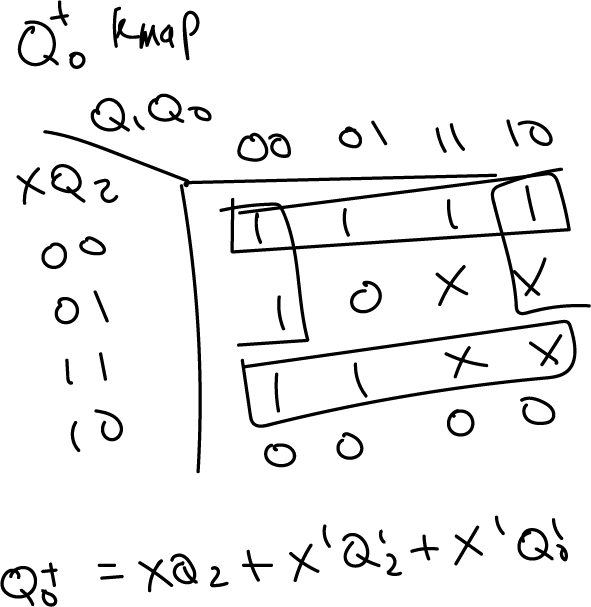
\includegraphics[scale=0.4]{Q4_Q0Kmap.png}
    \end{center}

    e) Complete the timing trace assuming each column is a new clock edge.

    \begin{center}
        \begin{tabular} {|c|c|c|c|c|c|c|c|c|c|}
            \hline
            X & 0 & 1 & 1 & 0 & 1 & 1 & 1 & 0 & ? \\
            \hline
            $Q_2$ & 0 & 0 & 0 & 1 & 0 & 0 & 1 & 1 & 1\\
            \hline
            $Q_1$ & 0 & 0 & 1 & 0 & 1 & 0 & 0 & 0 & 0\\
            \hline
            $Q_0$ & 0 & 1 & 0 & 0 & 1 & 0 & 0 & 1 & 0\\
            \hline
            $Z$ & 1 & 1 & 0 & 0 & 0 & 1 & 0 & 1 & 0\\
            \hline
        \end{tabular}
    \end{center}

    f) Design the combinational logic for the output Z using only one 4-to-1 multiplexer 
    and any other logic gates needed. Complemented variables are available. Draw the 
    multiplexer circuit and label all of your inputs.

    \begin{center}
        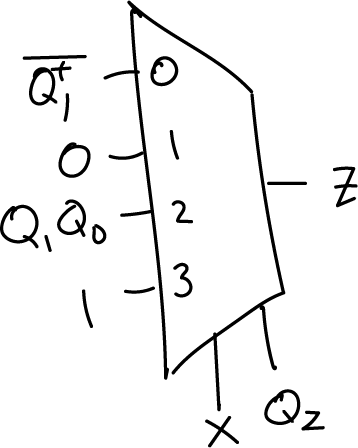
\includegraphics[scale=0.4]{Q4_4-1MUX.png}
    \end{center}

    %################################################################################### 
    
    \section*{Problem 5}

    Using the following circuit with input A and output Z:

    \begin{center}
        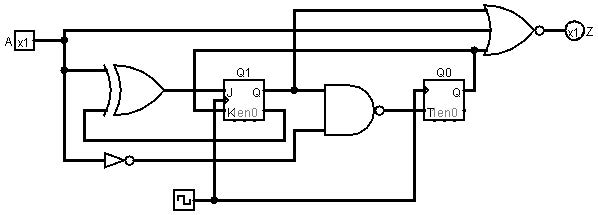
\includegraphics[scale=0.75]{Q5_Question.jpg}
    \end{center}

    (a) Is the above machine a Mealy or a Moore configuration? Why?

    \begin{enumerate}[label=\textbf{Solution:}, leftmargin=*]
        \item 
        This meachine is a Mealy configuration. This is because the output not only depends
        on the current state of the machine but also the present input.
    \end{enumerate}

    (b) Complete the timing diagram for the above circuit, assuming each flip flop 
    starts with an initial Q value of 0 and an active low clear (reset) is present. 
    Assume the clock uses a negative-edge triggering. You must show the outputs of each 
    of the flip-flops and the output Z (you do not need to show the J/K/T inputs).

    \textbf{Solution:}

    \begin{center}
        \begin{tabular} {c|l}
            Input/Output & Equation \\
            \hline
            $A$ & $A$ \\
            $J$ & $A\oplus \overbar{Q_1}$ \\
            $K$ & $Q_0$ \\
            $T$ & $\overbar{\overbar{A}Q_1}$ \\
            $Z$ & $\overbar{Q_1+Q_0+A}$ 
        \end{tabular}
        \quad
        \begin{tabular} {c|l}
            $JK$ & $Q_1^+$ \\
            \hline
            $00$ & $Q_1$ \\
            $01$ & $0$ \\
            $10$ & $1$ \\
            $11$ & $\overbar{Q_1}$
        \end{tabular}
        \quad
        \begin{tabular} {c|c|l}
            $T$ & $Q_0$ & $Q_0^+$ \\
            \hline
            $0$ & $0$ & $0$ \\
            $0$ & $1$ & $1$ \\
            $1$ & $0$ & $1$ \\
            $1$ & $1$ & $0$
        \end{tabular}
    \end{center}

    \begin{center}
        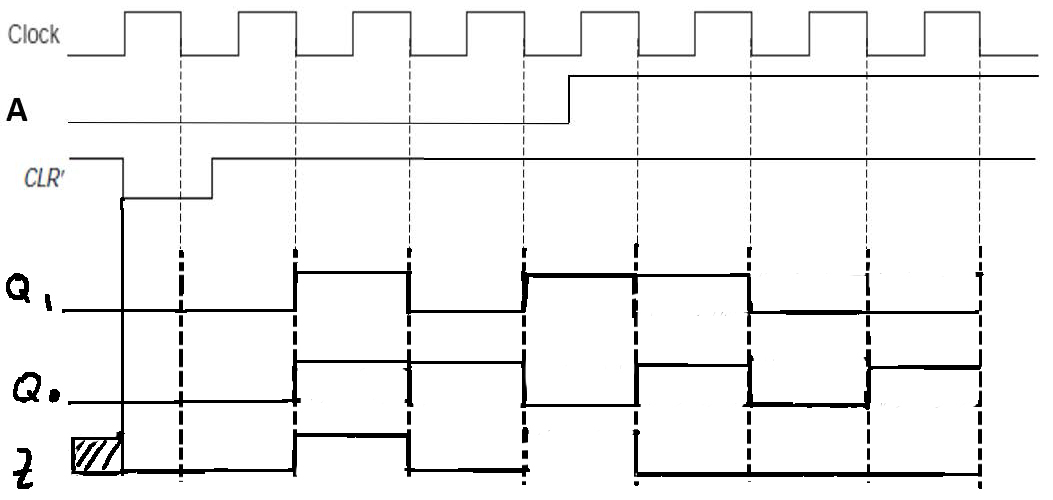
\includegraphics[width=\linewidth]{Q5_Question_b.jpg}
    \end{center}

    %################################################################################### 
    
    \section*{Problem 6}

    Redesign the Mealy Vending Machine (from the class lecture notes), to include an 
    output for providing “Change” if more than 15 cents is received instead of giving 
    credit, using only D flip flops and combinational logic.

    \begin{center}
        \begin{tabular} {|c|l|c|}
            \hline
            State & Definition & Binary ($Q_1$, $Q_0$) \\
            \hline
            $S_0$ & 0 cents deposited & $00$ \\
            $S_1$ & 5 cents deposited & $01$ \\
            $S_2$ & 10 cents deposited & $10$ \\
            $S_3$ & N/A & $11$ \\
            \hline
        \end{tabular}
    \end{center}

    Inputs = Dime (D), Nickel (N)

    Outputs = Vend (V), Change (C)

    Your design should show a state transition diagram, state transition table, K-maps, 
    and final minimum SOP equations for each D flip flop and each output.

    \textbf{Solution:}

    \begin{center}
        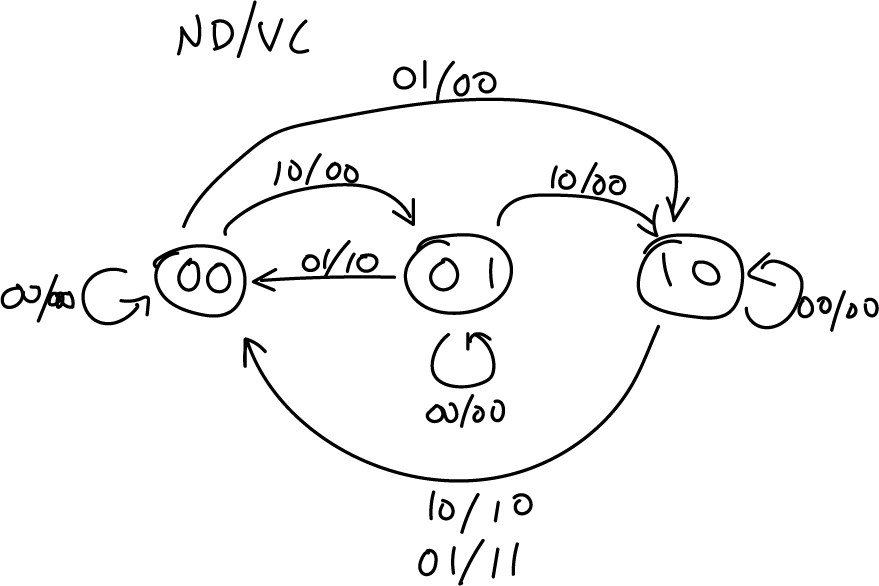
\includegraphics[scale=0.3]{Q6_State_diagram.png}
    \end{center}

    \begin{center}
        \begin{tabular} {c|c|c|c|c}
            ND & $Q_1Q_0$ & $Q_1^+Q_0^+$ & Vend & Change \\
            \hline
            00 & 00 & 00 & 0 & 0 \\
            00 & 01 & 01 & 0 & 0 \\
            00 & 10 & 10 & 0 & 0 \\
            00 & 11 & XX & X & X \\
            \hdashline
            01 & 00 & 10 & 0 & 0 \\
            01 & 01 & 00 & 1 & 0 \\
            01 & 10 & 00 & 1 & 1 \\
            01 & 11 & XX & X & X \\
            \hdashline
            10 & 00 & 01 & 0 & 0 \\
            10 & 01 & 10 & 0 & 0 \\
            10 & 10 & 00 & 1 & 0 \\
            10 & 11 & XX & X & X \\
            \hdashline
            11 & 00 & XX & X & X \\
            11 & 01 & XX & X & X \\
            11 & 10 & XX & X & X \\
            11 & 11 & XX & X & X \\
        \end{tabular}
    \end{center}

    \begin{center}
        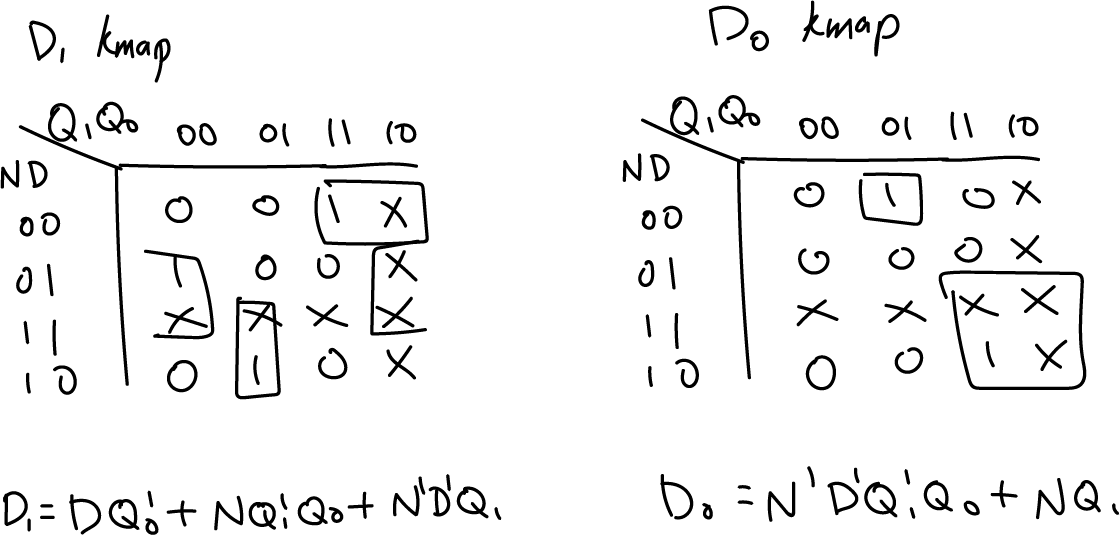
\includegraphics[scale=0.3]{Q6_DKmaps.png}
    \end{center}

    \begin{center}
        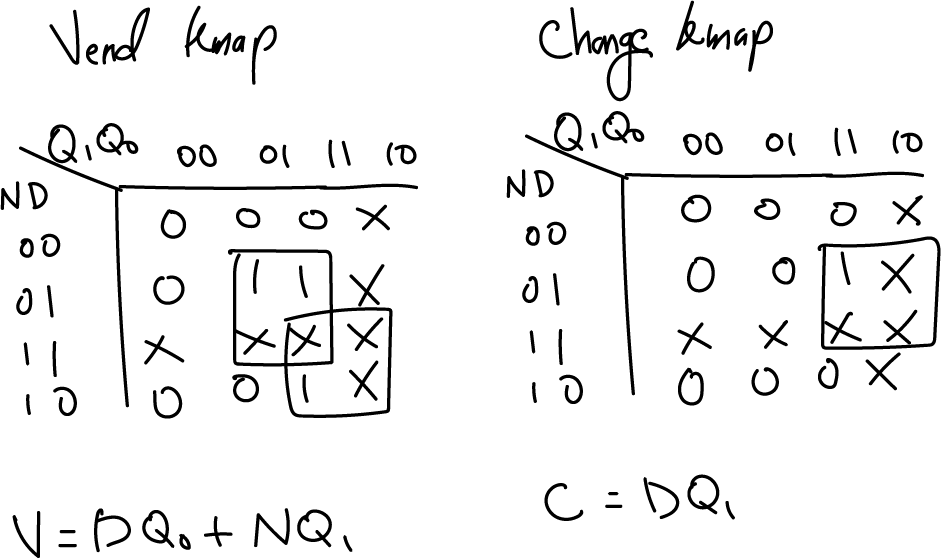
\includegraphics[scale=0.35]{Q6_OutKmaps.png}
    \end{center}

    %################################################################################### 
    
    \section*{Problem 7}

    Answer the following questions using your microprocessor design from Lab 4:

    (a) Write the binary program needed to be stored in the RAM to add the decimal values 
    7 and 12, then store the results in RAM location 15 (You may not need all 8 locations 
    of ROM).

    \begin{center}
        \begin{tabular} {|c|c|l|}
            \hline
            Address & Contents (Hex) & Comment \\
            Location & & \\
            \hline
            0 & 0x1205 & Load IR\\
            1 & 0x2234 & Read value and load it to ACC\\
            2 & 0x0294 & Reads value and adds it to ACC \\
            3 & 0x1205 & Load IR \\
            4 & 0x2304 & Reads address and loads MAR; increment PC\\
            5 & 0x000A & Loads ACC to data\_bus and writes to address\\
            6 & 0x1205 & Load IR \\
            7 & 0x1000 & STOP code \\
            \hline
        \end{tabular}
    \end{center}

    (b) Assuming both operands 7 and 12 are converted to 4 bit unsigned binary numbers, 
    what is the result of 7+12 if restricted to 4 bits? Show your answer in both 
    hexadecimal and binary with 4 bits. Does unsigned overflow occur?

    \textbf{Solution:}

    Yes, Unsigned overflow occurs.

    \begin{center}
        \begin{tabular} {ccccc}
            &   $0^1$ & $1$ & $1$ & $1$ \\
            $+$&$1$ & $1$ & $0$ & $0$ \\
            \hline
            overflow &$0$ & $0$ & $1$ & $1$
        \end{tabular}
        \quad
        \begin{tabular} {l}
            \text{hex: [7]} \\
            \text{hex: [C]} \\
            \text{hex: [3]}
        \end{tabular}
    \end{center}

\end{document}